\begin{surferPage}[30 Keerpunten]{Het zesdegraadsoppervlak van Barth met 30 keerpunten}
    Toen Wolf Barth het oppervlak van de zesde graad met het grootst mogelijke aantal singulariteiten had geconstrueerd, namelijk $65$ (zie elders in deze galerij), en twee van zijn doctoraatsstudenten ook nieuwe wereldrecords voor hogere graden hadden gevestigd, begon hij na te denken over het maximaal aantal keerpunten op oppervlakken van willekeurige graad.

   Barths constructie van het zesdegraadsoppervlak met $65$ singulariteiten van het type
    $A_1^{+-}$ (dubbele kegels) kan aangepast worden voor keerpunten, en dit geeft er $30$: 
    \[P_6 - \alpha \cdot K^3=0,\]
  waar $P_6$ dezelfde symmetrievlakken van de icosa\"eder zijn als bij het andere oppervlak van Barth, en waar $K$ opnieuw de vergelijking van het eenheidsboloppervlak is:
    \vspace*{-0.4em}
    \begin{center}
      \begin{tabular}{c@{\ }c@{\ }c@{\ }c}
        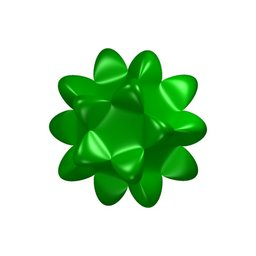
\includegraphics[height=1.2cm]{barthsextic_30A2}
        &
        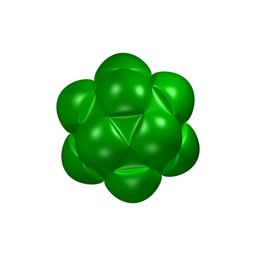
\includegraphics[height=1.2cm]{barthsextic_30A2_3}
        &
        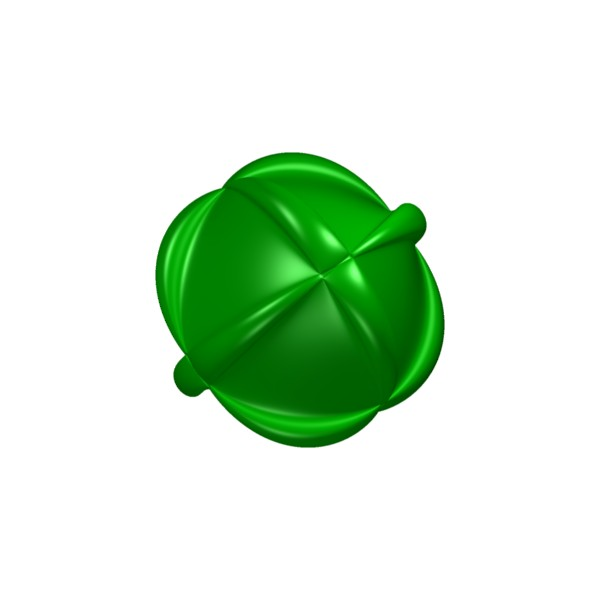
\includegraphics[height=1.2cm]{barthsextic_30A2_5}
        &
        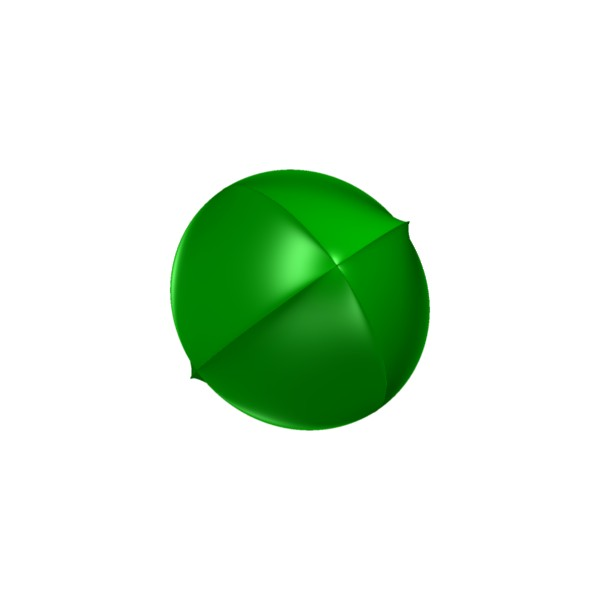
\includegraphics[height=1.2cm]{barthsextic_30A2_6}
      \end{tabular}
    \end{center}    
    \vspace*{-0.3em}
     Dit is het huidige wereldrecord wat het aantal re\"ele keerpunten op zesdegraadsoppervlakken betreft. Voor complexe keerpunten is het record $36$.
\end{surferPage}
